\documentclass[class=minimal,border=0pt]{standalone}
\usepackage{tikz}
\usepackage{amsmath}

\usetikzlibrary{%
  arrows,
  calc
}
\usetikzlibrary{decorations.markings}
\usetikzlibrary{shapes.misc}

\begin{document}
  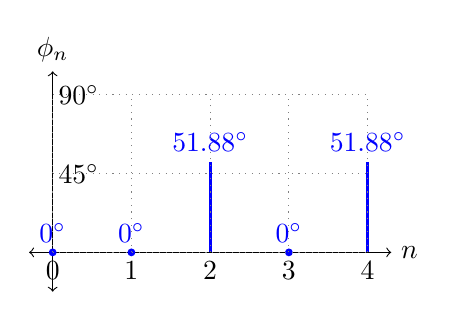
\begin{tikzpicture}[yscale=1, xscale=1]
    \draw[<->] (-0.3,0) -- (4.3,0) node[right] {$n$};
    \draw[<->] (0,-0.5) -- (0,2.3) node[above] {$\phi_n$};
    
    %Values
    
    \node at (0,0) [circle,fill,inner sep=1pt,blue]{};
    \draw (0,0) node[blue,above] {$0^{\circ}$};
    \node at (1,0) [circle,fill,inner sep=1pt,blue]{};
    \draw (1,0) node[blue,above] {$0^{\circ}$};
    \draw[-,line width = 1pt, blue] (2,0) -- (2,1.153);
    \draw (2,1.153) node[blue,above] {$51.88^{\circ}$};
    \node at (3,0) [circle,fill,inner sep=1pt,blue]{};
    \draw (3,0) node[blue,above] {$0^{\circ}$};
    \draw[-,line width = 1pt, blue] (4,0) -- (4,1.153);
    \draw (4,1.153) node[blue,above] {$51.88^{\circ}$};
     
    % x-Axis scale
    \draw (0,0) node[below] {$0$};
    \draw (1,0) node[below] {$1$};
    \draw (2,0) node[below] {$2$};
    \draw (3,0) node[below] {$3$}; 
    \draw (4,0) node[below] {$4$};
  
	% y-Axis Scale
    \draw (-0.05,2) node[right] {$90^{\circ}$};
    \draw (-0.05,1) node[right] {$45^{\circ}$};
  
    %Grid
    \draw[dotted,step=1cm,color=gray,thin] (0,0) grid (4,2);

  \end{tikzpicture}

\end{document}